\documentclass[review]{elsarticle}

%\usepackage{amssymb}
\usepackage{amsmath}
\usepackage{graphicx}
%\usepackage[figuresright]{rotating}
\usepackage{subfigure}
%\usepackage{wrapfig}
\usepackage{tikz,pgf}
\usetikzlibrary{arrows}

\usepackage{lineno,hyperref}
\modulolinenumbers[5]
\bibliographystyle{elsarticle-num}

\usepackage{color}

\begin{document}

\begin{frontmatter}
  
\title{Mesh generation with adaptive refinement using hash tables}
\author[1]{Priscila Cardoso Calegari \corref{email}}
\address[1]{Departamento de Computa\c{c}\~ao, Universidade Federal de Santa Catarina, Ararangu\'a, SC, Brazil}
\cortext[email]{Corresponding author}
\ead{priscila.calegari@ufsc.br}
\author[2]{\'Alvaro Junio Pereira Franco}
\address[2]{Departamento de Inform\'atica e Estat\'istica, Universidade Federal de Santa Catarina, Florian\'opolis, SC, Brazil}

\begin{abstract}
In this work we have presented a tool to generate meshes with adaptive and dynamic refinement. A hash table is used to manage the mesh elements and for searching, insertion, deletion, refine, and coarsening. The numerical experiments was performed in two-dimensional meshes with many different refinement levels. We present results in the mesh generation for simulating the vortex sheet.
\end{abstract}

\begin{keyword} 
  Mesh generation \sep Adaptive Mesh Refinement \sep Hash Table \sep Refinement and merger operations
  \end{keyword}
\end{frontmatter}

\linenumbers

\section{Introduction}\label{sec-introduction}

Adaptive mesh refinement is a wide and fundamental technique in numerical simulation of several physical problems. Between them we can highlight, problems that involve combustion, phase separation, deformation of drops, particle transport, wave propagation, and fluid-structure interaction \cite{ROM99,DUA13,PEM98,BER84,BEL05,CEC10,WEL15}. The idea is concentrate computational power in regions of interest. The computational domain discretization is based on Adaptive Mesh Refinement (AMR) proposed by Berger and Oliger \cite{BER84} and Berger and Collela \cite{BER89}. The technique deals with dynamic problems (with time evolution) and the localized refinement decreases the computational cost. The mesh refinement in regions of interest adapts based on predetermined criteria. There is many different mesh proposals. Some triangulate the domain. Others partition the domain in squares or rectangles (cells) and those that are composed by visible cells and not visible cells (ghost cells) \textcolor{red}{here some reffereces}. The adaptive mesh refinement, proposed here, stores only information of visible cells. 
 
In this work we present a tool that generates meshes using a hash table as a data structure for managing the storage of its cells. This structure allows \emph{insert}, \emph{remove}, and \emph{retrieve} cells in an efficient way. The expected time spent in each operation is constant. Moreover, we can refine a cell, or merge some cells in one cell. This allows us changing a mesh in the exact moment that one cell needs to be refined or some cells need to be merged. Thus a phase performed for some numerical simulation tool, that remap a mesh in time $t_i$ for a mesh in time $t_{i+1}$ (see for example \cite{COL18}), is not necessary anymore.

The storage management of the mesh cells should be done by some data structure. A simple list can be used. However, retrieve a cell, without knowing exactly where is it in the list, it is an expensive operation. If the mesh has $N$ stored cells in the list, then the execution time is $O(N)$. For this case, insert a cell can be done quickly ($O(1)$, constant time), for example, as long as the insertion is done at the beginning of the list. Remove also can be done quickly ($O(1)$ time), if the location cell in the list is known. Other data structures generally used are based on \emph{trees} such as \emph{kd-trees} and \emph{quadtrees} or \emph{octrees} \textcolor{red}{\cite{}}. However, the insert, delete, and retrieve operations depend on the height of the tree, which is $\Omega(\log N)$ where $N$ is the cell number stored in the tree. Here, with the hash table, the \emph{expected time} to insert, delete, and retrieve the cell is $O(1)$. In literature, some studies have already used od hash tables. \textcolor{red}{\cite{COL18}. \cite{GRI99}. \cite{MUL03}.}

The outline of the paper is as follows. Section~\ref{sec-AMR} presents the adaptive mesh refinement technique. Section~\ref{sec-ED} presents the fundamental operations defined in the mesh with the hash table data structure. Section~\ref{sec-results} presents the numerical experiments. The conclusions are presented in Section~\ref{sec-conclusions}.
 

%%%%%%%%%%%%%%%%%%%%%%%%%%%%%%%%%%%%%%%%%%%%%%%%%%%%%%%%%%%%%%%%%%%%%%

\section{Adaptive mesh refinement generation}\label{sec-AMR}


This work considers meshes that discretizes two-dimensional computational domain. However, it is possible generalize the results for three-dimensional meshes. First of all, we have generated a uniform mesh that covers a domain $[a_1,b_1]\times[a_2,b_2]$. This uniform mesh is called base level and it is composed by rectangular cells. The cell center is given by cartesian coordinates $(x_i,y_i) = (a_1 + (i + \frac{1}{2})\Delta x), a_2 + (j + \frac{1}{2})\Delta y))$, with $\Delta x = (b_1 - a_1)/N$, $\Delta y = (b_2 - a_2)/M$, and $N, M$ are cell numbers in each of the directions $x$ and $y$, respectively. 

From a uniform mesh, we initiate the refinement process in a particular region of interest, where each selected cell is divided and replaced by four new cells.  The process continues, until it is reached the maximum refinement level $L$. A refinement level $l$ is composed by a set of cells that have tha same dimensions, $\Delta x^l$ and $\Delta y^l$, where $\Delta x^l = 2\Delta x^{l+1}$ and $\Delta y^l = 2\Delta y^{l+1}$. The refinement ratio is given by $\Delta x^{l}/\Delta x^{l+1} = 2$ where $l$ is an non negative integer number. Each cell $c$ of a mesh is uniquely identified by three elements $c = (i, j, l)$, where $i$ and $j$ are the coordinate index, $x$ and $y$, respectively, and $l$ is the refinement level. Figure~\ref{fig1} presents a meshes generated by this technique with $\Delta x^l = \Delta y^l$.  

\begin{figure}[htb]
  \begin{center}
    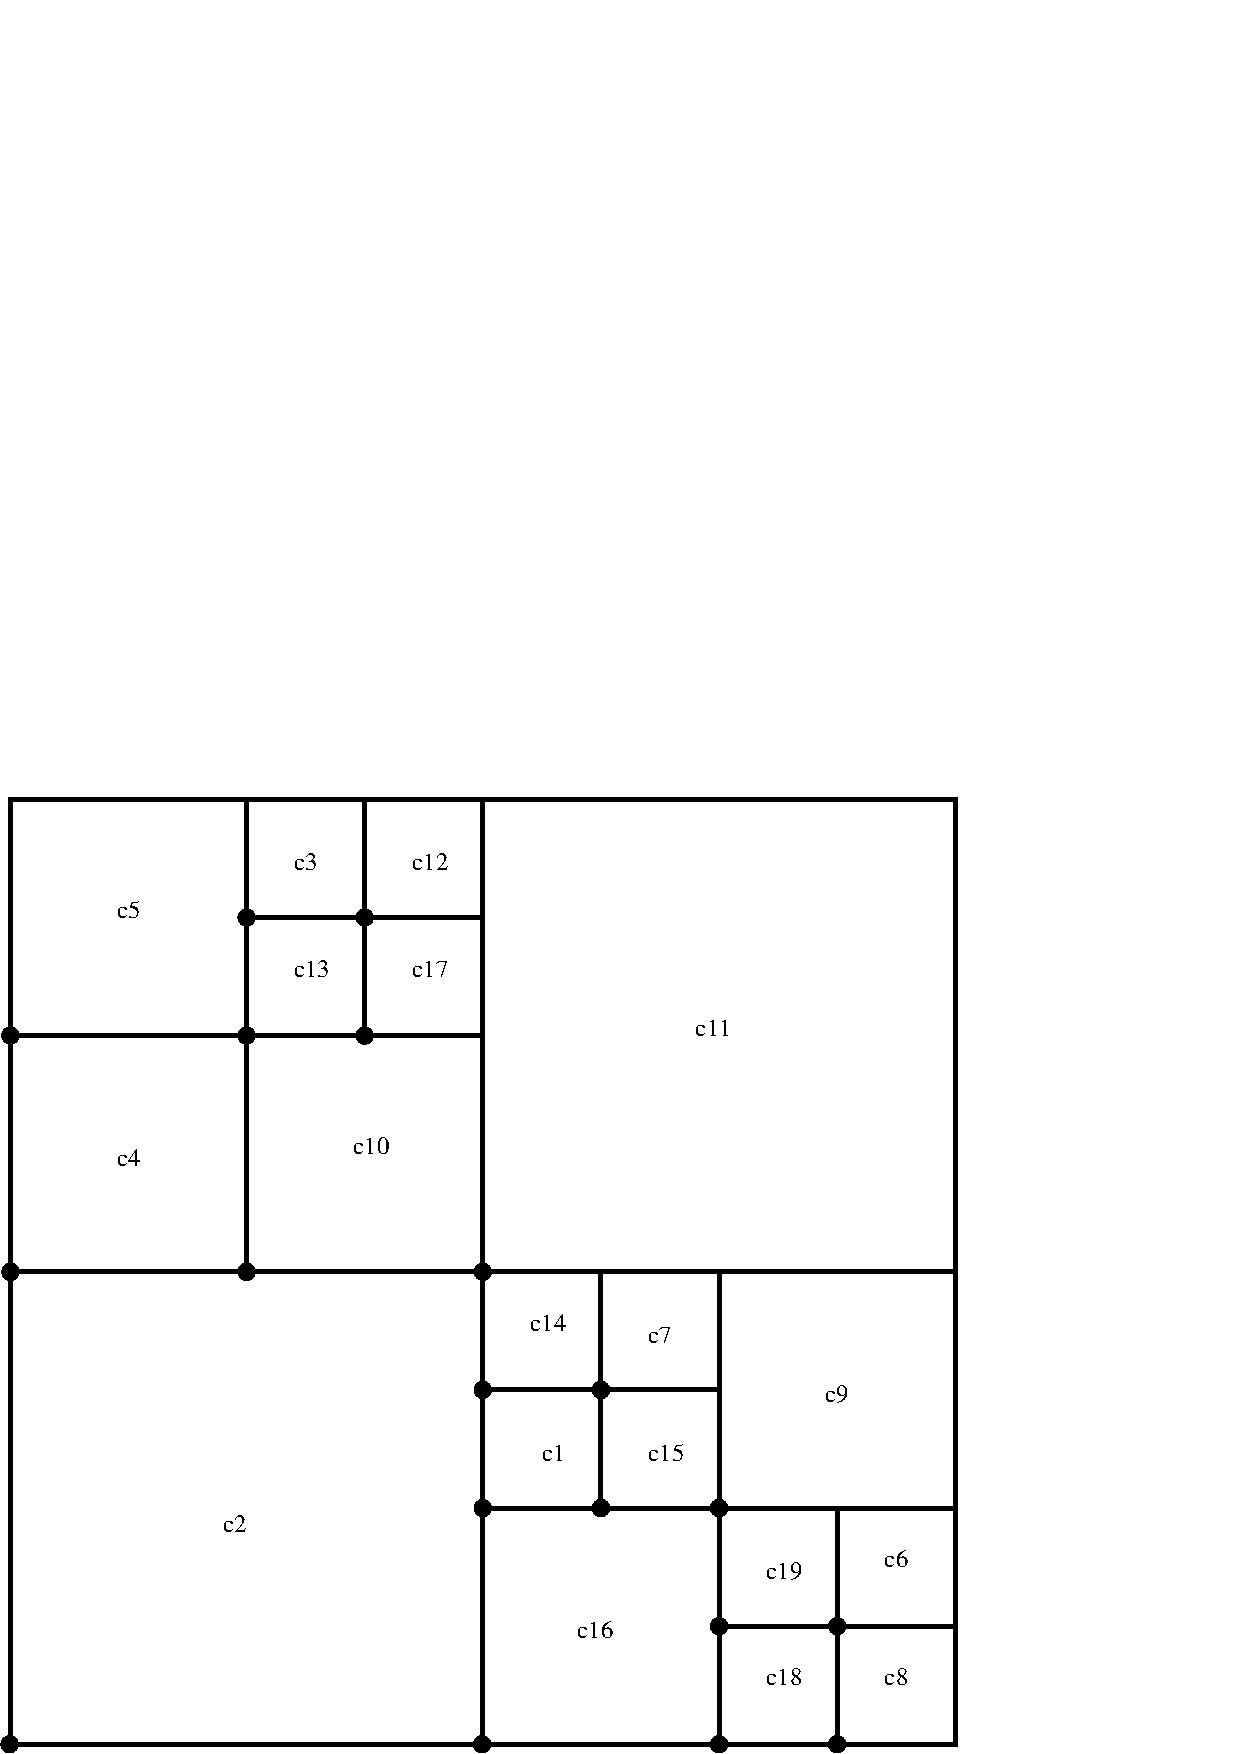
\includegraphics[width=0.43\textwidth]{figure/exemplo-malha.pdf}
    \put(-113,37){{\scriptsize $c_1$}}
    \put(-42,109){{\scriptsize $c_2$}}
    \put(-59,19){{\scriptsize $c_3$}}
    \put(-23,55){{\scriptsize $c_4$}}
    \put(-132,92){{\scriptsize $c_5$}}
    \put(-95,92){{\scriptsize $c_6$}}
    \put(-132,129){{\scriptsize $c_7$}}
    \put(-33,9){{\scriptsize $c_8$}}
    \put(-13,9){{\scriptsize $c_9$}}
    \put(-14,28){{\scriptsize $c_{10}$}}
    \put(-34,28){{\scriptsize $c_{11}$}}
    \put(-71,46){{\scriptsize $c_{12}$}}
    \put(-51,46){{\scriptsize $c_{13}$}}
    \put(-51,66){{\scriptsize $c_{14}$}}
    \put(-71,66){{\scriptsize $c_{15}$}}
    \put(-107,120){{\scriptsize $c_{16}$}}
    \put(-88,120){{\scriptsize $c_{17}$}}
    \put(-88,138){{\scriptsize $c_{18}$}}
    \put(-107,138){{\scriptsize $c_{19}$}}
  \end{center}
  %\vspace{-1.5pc}
  \caption{\small Adaptive mesh with three refinement levels.}
  \label{fig1}
\end{figure}

In the construction process of the adaptive and dynamic mesh, we have defined two operations: {\em refine} and {\em coarsening}. Assume the following instance: in a given instant of time a certain region of domain can be considered less important for solving the problem. Thus, the mesh should be coarser in this region. Or else, in the course of time, such region is important and then it must be refined. As an example, we have considered the Figure~\ref{fig1}, to describe this two operations. Cells $c_{16}$, $c_{17}$, $c_{18}$, and $c_{19}$ (called siblings cells) are generated of a refinement process of a cell, whose area coincides with total area of this four cells. Therefore, given a cell $c = (i, j, l)$, where $l$ is smaller than the finest level, the operation {\em refine} divides $c$ in four new cells: $c_{16}=(2i, 2j, l+1)$, $c_{19}=(2i, 2j + 1, l+1)$, $c_{17}=(2i+1, 2j+1, l+1)$, and $c_{18}=(2i+1, 2j, l+1)$. Cell $c$ is removed of the mesh and the four new cells are inserted. As the number of insertions and deletions in hash table used by this operation is constant, the expected execution time of this operation depends on the expected time of insertion and deletion in hash table (next we will see that both expected time are constant). Following two another important points. First of all, the $c$ coordinates are integers number, then the cells coordinate resulting of operation also will be integers. The advantage is that operation is not subject to numerical errors. Second point is related to parity of coordinates obtained in refine operation by sibling cells. Note that bottom left cell, for example $c_{16}$, always has even indexes; while a top right cell, for example $c_{18}$, always has odd indexes. Already {\em coarsening} operation performs the inverse of {\em refine} operation. {\em Coarsening} operation transforms four sibling cells, all in the same level $l$, in a cell in the level $l - 1$, where $l > 0$ ($0$ is the level of base mesh). This transformation will be effective only if all sibling cells exist in mesh. Otherwise, the operation is not performed. Once again, we have a constant number of insertion and deletion of cells in hash table for this operation. Thus, expected time for coarsening is constant. Figure~\ref{fig2} shows a adaptive mesh randomly generated with five refinement levels. Next, data structure hash table is briefly described.

\begin{figure}[htb]
  \begin{center}
     \includegraphics[width=0.5\textwidth]{figure/malha1.pdf}
    %\hspace{0.5pc}
    \includegraphics[width=0.455\textwidth]{figure/malha2.pdf}
    \put(-80,-8){{\scriptsize (b)}}
   \put(-248,-8){{\scriptsize (a)}} 
  \end{center}
  %\vspace{-1.5pc}
  \caption{\small (a) Adaptive mesh randomly generated and (b) zoom of a region.}
  \label{fig2}
\end{figure}

\section{Hash Table data structure}\label{sec-ED}

\textcolor{red}{Incluir algumas figuras.}

Hashing technique is a useful way to store and retrieve data items in a table, that is efficient in both time and space \cite{BEN15,DAS08,CLRS09}. Here, we have used a hash table to store cells of meshes. It is worth mentioning that refinement process is adaptive and dynamic. Thus, we have expected many insertion and deletion of cells while new meshes are generated. Insert, search and delete operation should be performed quickly. In hash tables, this operations consume expected time constant. In the worst-case, the time consumed of each operation is $O(N)$, where $N$ is the number of elements stored in table \cite{CLRS09,KNU97,SZW12}. However, such time probably will not occur if we assure a good dispersion of elements in table. Thus, for efficiency to be satisfactory in hash table, is necessary a hash function that contributes with a low number of key collisions. Note that a collision occurs when two or more different keys have the same value returned by a hash function. 

%%%%%%%%%%%%%%%%%%%%%%%%%%%%%%%%%%%%%%%%%%%%%%%%%%%%%%%%
Each cell has a key given by its level and indexes of coordinates vertex. In this way, all key is unique, in other words, there are no two different cells with the same key. The key of a cell is used to obtain a index of table where a corresponding cell will be stored. For this, is used a {\em hash function}, that receives the key of a cell $c$ and returns a index of tha table for $c$. Hash function can be not injective. Thus, the function can returns the same index table for two keys of different cells, this is called collision. In this case, we have needed a mechanism to treat collisions. Here, the collisions in hash table were treated with lists. This means that two different cells can be stored in a list that is associated with a unique table index. Experimentally, we have observed that hash function given by Fibonacci's method \cite{KNU97} presents a good behaviour. There are theoretical results that guarantee expected time constant for insert, delete, and search operation in hash table. For this, we have to assume that hash function spreads uniformly the cells. Moreover, we have to keep the quantity of table position, for example, lightly larger than double of cell number that we want store.

%%%%%%%%%%%%%%%%%%%%%%%%%%%%%%%%%%%%%%%%%%%%%%%%%%%%%%%%%%%%%%%%
 The fundamental operations of the hash table were implemented. The insertion operation of a new cell in hash table receives a new cell $c$, computes its key $K$, and stores $c$ in the position returned by hash function applied on $K$. The deletion operation receives a cell $c$, computes its key, uses a hash function to get the position of $c$ in hash table, and removes $c$, if it exists. The retrieve operation receives the indexes and the level of a cell, computes its key, and the position where a cell with such characteristics should be, and returns such cell, if it exists. As previously mentioned, the expected execution for each operation is constant. Next we have described our numerical experiments.

%%%%%%%%%%%%%%%%%%%%%%%%%%%%%%%%%%%%%%%%%%%%%%%%%%
\section{Numerical Experiments}\label{sec-results}

In the first numerical experiment, we have generated a refined mesh for the initial condition of the drop deformation (see \cite{CEC10,WEL15}). Here, the mesh is two-dimensional domain $[a_1,b_1]\times[a_2,b_2]$, with $a_1=a_2=0$ and $b_1=b_2=1$. The initial condition is given by,
\begin{equation}\label{eq1e1}
  \phi(x,y)=\tanh[\alpha(r - d)],
\end{equation}
where $\alpha = 75$, $r=0.25$ the circumference radius, $d=\sqrt{(x-x_c)^2+(y-y_c)^2}$ the distance between each point $(x,y)$ of domain, and the circumference center $(x_c,y_c)=(0.5,0.5)$. Figure~\ref{figA1} presents the function $\phi$ and the adaptive mesh with five refinement levels.
\begin{figure}[!ht]
  \begin{center}
    \includegraphics[width=0.48\textwidth]{figure/gota.pdf}
    \hspace{0.5pc}
    \includegraphics[width=0.48\textwidth]{figure/gotaref.pdf}
    \put(-80,8){{\scriptsize (b)}}
    \put(-255,8){{\scriptsize (a)}}
  \end{center}
  \vspace{-1.5pc}
  \caption{{\small Function $\phi(x,y)$ evaluated in adaptive mesh with five refinement levels and base level with $32\times 32$ cells.}}
  \label{figA1}
\end{figure}

We have generated meshes with base level $32\times 32$ cells and some different refinement levels. The refinement criterium was the same for all cases. The refined cells were those who satisfied $-0,99 < \phi(x,y) < 0,99$.

Table~\ref{tab1} presents information of the hash table, like level number of mesh ($L$), cell number of mesh ($N$), number of positions in hash table ($P$), appoximated load factor ($N/P$), collisions number ($C$), maximum number of cells per table position ($CMAX$), and lower limit for the height of any binary tree that stores $N$ cells ($\lfloor\log_2(N)\rfloor$).% e o número de remoções.

\begin{table}[ht]\label{tab1}
\caption{ {\small Hash table information.}}
\centering
\begin{tabular}{ccccccc}
  \hline
$L$  & $N$  & $P$ & $N/P$ & $C$ & $CMAX$ & $\lfloor\log_2(N)\rfloor$ \\%& colisões $20\%$ & cmax ($20\%$) \\  
\hline
3  &2.488 & 1.638  & 1,52 & 1.691 &  7 & 11 \\%& 1285 & 6 \\
4  &5.500 & 6.553  & 0,84   & 1.717 & 4 & 12  \\%& 1238 & 3\\
5  &15.772 & 26.214 & 0,60 & 6.882 & 5 & 13 \\ %& 3900 & 4 \\%& 20688 \\
6  &51.808 & 104.857 & 0,49  & 16.928 & 4 & 15 \\%& 10271 & 3\\
7  &179.512 & 419.430 & 0,43  & 63.238 & 5 & 17 \\%& 33659 & 3 \\
\hline
\end{tabular}\label{tab1}
\end{table}

The number of positions in the hash table is nearly $10\%$ of the cell number of a uniform mesh equivalent to finest level. For example, in the experiment with three refinement levels ($L3$) and base level with $32 \times 32$ cells, the cell number of a mesh equivalent to finest level is $128 \times 128 = 16.384$ cells (see first column and column $P$ in table~\ref{tab1}). %O número de inserções realizadas na tabela de dispersão é igual ao número de células mais o número de remoções.}

It is important to note in Table~\ref{tab1} that load factor for $L3$ is bigger than one. This means that there are more cells than positions in hash table. The collisions number in mesh $L3$ was about $68\%$ of total cell number, while for meshes $L4$ and $L6$ were about foram $31\%$ and $33\%$, respectively. Moreover, note that maximum cell number in a position of hash table always have been smaller than height of any binary tree. Figure~\ref{figE1} presents others statistical results of hash table for each mesh in Table~\ref{tab1} ($L3$ until $L7$). Here, we have computed the collision rate, occupation rate, and vacancy rate.

\textcolor{red}{Alterar a figura.}
\begin{figure}[!ht]
  \begin{center}
        \includegraphics[width=0.49\textwidth]{figure/vaziaxocupada2.pdf}
    \includegraphics[width=0.49\textwidth]{figure/ocupadas2.pdf}
    \put(-90,-8){{\scriptsize (b)}}
    \put(-262,-8){{\scriptsize (a)}}
  \end{center}
  \vspace{-1pc}
  \caption{{\small Statistical results: (a) Collisions by cell number, occupation rate, and vacancy rate in the hash table and (b) Cell number that occupy $k$ positions in the hash table.}}
  \label{figE1}
\end{figure}

Figure~\ref{figE1}(a) presents the ratio between collision number and cell number ($C/N$), the ratio between number of empty positions ($E$) and table size ($P$), and the ratio between number of occupied positions ($O$) and table size for each mesh ($L3, L4,\dots, L7$). Among all meshes, the maximum number of cells in the same position of hash table have been $7$ cells. The mesh $L3$ was the only one who presented $6$ and $7$ cells that occupy the same cell. Figure~\ref{figE1}(b) presents the ratio between a position with $k$ cells, for $k=1,2,\ldots,5$, and the total number of positions in hash table. In this computation it was considered all positions of hash table, including the positions with empty lists. Thus, $L4$ has tha largest proportion of $1$ cell by position of hash table and the cell number by position decreases quickly. Moreover, mesh $L4$ has been presented the best cost/benefit compared to load factor $84\%$, vacancy rate $42\%$, and occupation rate $58\%$.

%\begin{table}[ht]
%\caption{ {\small Tabela de dispersão malha base $16\times 16$.}}
%\centering
%\begin{tabular}{cccccccc}
%\toprule
%L  & m  & n & n/m & c & nmax & remoções & inserções\\ \midrule
%4  & 3276  & 1336  & 0.40 & 401  & 4 & 360  & 1696 \\
%5  & 13170   & 3724  & 0.28  & 716 & 3 & 1156 & 4880\\
%6  & 52428 & 12352  & 0.23 & 2470 & 3 & 4032 & 16384 \\
%7  & 209715 & 43636   & 0.20  & 7826 & 3 & 14460 & 58096\\
%\bottomrule
%\end{tabular}\label{tab2}
%\end{table}

%\begin{table}[ht]
%\caption{ {\small Tabela de dispersão malha base $64\times 64$.}}
%\centering
%\begin{tabular}{ccccc}
%\toprule
%L  & m  & n & n/m & c \\ \midrule
%3  & 13170 & 9760  & 0.74   &  3  \\
%4  & 52428   & 21796  & 0.41   & 4 \\
%5  & 209715 & 63160  & 0.30 & 3  \\
%6  & 838860 & 207616   & 0.24  & 3 \\
%7  & 3355443 & 719296  & 0.21  & 3 \\
%\bottomrule
%\end{tabular}\label{tab3}
%\end{table}

The second numerical experiment is a simulation of Kelvin-Helmholtz instability \cite{DUA13,CEC10}. The purpose of this experiment is to show the dynamics of the adaptive mesh. For this, we have included the transport of lagrangian particles, modeled by the ODE system,
\begin{equation}\label{eq1}
 \begin{array}{l}
    \dfrac{d}{dt}x_p(t) = u(t,x_p,y_p),\\ \\%\dfrac{(y_p-y_c)vt(d,t)}{d}, \hspace{.5cm}
    \dfrac{d}{dt}y_p(t) = v(t,x_p,y_p),%-\dfrac{(x_p-x_c)vt(d,t)}{d},
  \end{array}
\end{equation}
where $(x_p,y_p)$ is the particle position in the computational domain. The velocity field is analytically defined by,
\begin{equation}\label{eq2}
  \begin{array}{l}
    u(t,x,y) = \dfrac{(y-y_c)vt(d,t)}{d},\\ \\
    v(t,x,y) = -\dfrac{(x-x_c)vt(d,t)}{d},
  \end{array}
\end{equation}
where $vt(d,t) = (A/2\pi d)(1 - e^{-d^2/4\mu t})$, with $A = 500$, $\mu = 10$, $(x_c,y_c)=(0,0)$, and $d=\sqrt{(x-x_c)^2+(y-y_c)^2}$.  The computational domain is $[a_1,b_1]\times[a_2,b_2]$ with $a_1=a_2=-0.5$ and $b_1=b_2=0.5$, and initially $1.000$ particles are distributed along the axis $x$ (with a slight perturbation, see Figure~\ref{figA2}). The Runge-Kutta's method of fourth order was used to obtain the numerical solution of the ODE system (\ref{eq1}). The refinement criterium to generate the dynamic mesh was the particle position. The base level has $32\times32$ cells and four refinement levels. Figure~\ref{figA2} presents the numerical solution in a few time step.   

\textcolor{red}{alterar a figura}
\begin{figure}[!ht]
  \begin{center}
    \includegraphics[width=0.49\textwidth]{figure/visit0371.pdf}
    \includegraphics[width=0.49\textwidth]{figure/visit0027.pdf}
    \vspace{-2pc}
    \includegraphics[width=0.49\textwidth]{figure/visit0365.pdf}
    \includegraphics[width=0.49\textwidth]{figure/visit0250.pdf}
    \vspace{-2pc}
    \includegraphics[width=0.49\textwidth]{figure/visit0188.pdf}
    \includegraphics[width=0.49\textwidth]{figure/visit0187.pdf}
  \end{center}
  %\vspace{-1.5pc}
  \caption{{\small Simulação da instabilidade de Kelvin-Helmholtz.}}
  \label{figA2}
\end{figure}

%O fator de ocupação da tabela de dispersão variou de $14\%$ a $25\%$. A variação do número máximo de células em uma posição da tabela foi de duas a quatro. O número de colisões varia de 40 a 250.  
 
\section{Concluding remarks}\label{sec-conclusions}

In this work, we have presented a adaptive mesh generator using hash tables. Hash function and the way to treat collisions are classical, but they has soma advantages and theoretical guarantees. For example, if $P$ is $O(N)$ and the function spreads uniformly the cells in hash table, then the expected number of cells in one position of table is constant \cite{CLRS09}. It is important to remember that there is no more than $7$ cells in one position of any hash table in our experiments. Moreover, the implementation of this proposed is simple and fast. However, there are hash functions that are \emph{perfects}, that is, this functions guarantee maximum one cell by position of table, without collisions. It is important verify the efficiency of such functions in numerical experiments. To finish, the operations \emph{refine} and \emph{coarsening} allow the mesh modification \emph{online}, without being necessary remap one mesh on another. Thus, it is expected a gain in execution time when compared to other methods that consider this remap. 

%----------------------------------------------------------
\section*{Acknowledgments}
{\small
\noindent  For their valuable discussions and helpful insights, the authors are in debt with Dr. Alexandre Megiorin Roma and Dra. Catalina Maria Rua Alvarez. Financial support was provided by CNPq grants \# 423833/2018-9.} %The authors thank the reviewers for their valuable comments and suggestions.

\section*{References}

\bibliography{mybibfile}

\end{document}




